% arara: pdflatex: { synctex: yes }
% arara: makeindex: { style: ctuthesis }
% arara: bibtex

% The class takes all the key=value arguments that \ctusetup does,
% and a couple more: draft and oneside
\documentclass[oneside]{ctuthesis}
\usepackage{siunitx}
\usepackage{nomencl}
\usepackage{setspace}
\usepackage{indentfirst}

%%%%%%%%%%%%%%%%%% insert images from other directory
\usepackage{graphicx}
\graphicspath{{./images/}}

%%%%%%%%%%%%%%%%%%%%%%%%%%%%%%%%%%%%%% this shit is here to break long url into more lines
\usepackage{url}
\makeatletter
\g@addto@macro{\UrlBreaks}{\UrlOrds}
%\makeatother

%%%%%%%%%%%%%%%%%%%%%%%%%%%%%%%%%%%%%% this shit is here to prevent breaking words on the edge of a line
\tolerance=1
\emergencystretch=\maxdimen
\hyphenpenalty=10000
\hbadness=10000


%%%%%%%%%%%%%%%%%%%%%%%%%%.this makes the differed text make different
%DIF PREAMBLE EXTENSION ADDED BY LATEXDIFF
%DIF UNDERLINE PREAMBLE %DIF PREAMBLE
\RequirePackage[normalem]{ulem} %DIF PREAMBLE
\RequirePackage{color}\definecolor{RED}{rgb}{1,0,0}\definecolor{BLUE}{rgb}{0,0,1} %DIF PREAMBLE
\providecommand{\DIFadd}[1]{{\protect\color{blue}\uwave{#1}}} %DIF PREAMBLE
\providecommand{\DIFdel}[1]{{\protect\color{red}\sout{#1}}}                      %DIF PREAMBLE
%DIF SAFE PREAMBLE %DIF PREAMBLE
\providecommand{\DIFaddbegin}{} %DIF PREAMBLE
\providecommand{\DIFaddend}{} %DIF PREAMBLE
\providecommand{\DIFdelbegin}{} %DIF PREAMBLE
\providecommand{\DIFdelend}{} %DIF PREAMBLE
%DIF FLOATSAFE PREAMBLE %DIF PREAMBLE
\providecommand{\DIFaddFL}[1]{\DIFadd{#1}} %DIF PREAMBLE
\providecommand{\DIFdelFL}[1]{\DIFdel{#1}} %DIF PREAMBLE
\providecommand{\DIFaddbeginFL}{} %DIF PREAMBLE
\providecommand{\DIFaddendFL}{} %DIF PREAMBLE
\providecommand{\DIFdelbeginFL}{} %DIF PREAMBLE
\providecommand{\DIFdelendFL}{} %DIF PREAMBLE
%DIF END PREAMBLE EXTENSION ADDED BY LATEXDIFF



% to print code
\usepackage{listings}
\usepackage{color}
\definecolor{dkgreen}{rgb}{0,0.6,0}
\definecolor{gray}{rgb}{0.5,0.5,0.5}
\definecolor{mauve}{rgb}{0.58,0,0.82}
\lstset{frame=tb,
  language=Java,
  aboveskip=3mm,
  belowskip=3mm,
  showstringspaces=false,
  columns=flexible,
  basicstyle={\small\ttfamily},
  numbers=none, 
  % numberstyle=\tiny\color{gray},
  % keywordstyle=\color{blue},
  % commentstyle=\color{dkgreen},
  % stringstyle=\color{mauve},
  breaklines=true,
  breakatwhitespace=true,
  tabsize=3
}
% to display source code
\definecolor{mGreen}{rgb}{0,0.6,0}
\definecolor{mGray}{rgb}{0.5,0.5,0.5}
\definecolor{mPurple}{rgb}{0.58,0,0.82}
\definecolor{backgroundColour}{rgb}{0.95,0.95,0.92}
\lstdefinestyle{CStyle}{
    backgroundcolor=\color{backgroundColour},   
    commentstyle=\color{mGreen},
    keywordstyle=\color{magenta},
    numberstyle=\tiny\color{mGray},
    stringstyle=\color{mPurple},
    basicstyle=\footnotesize,
    breakatwhitespace=false,         
    breaklines=true,                 
    captionpos=b,                    
    keepspaces=true,                 
    numbers=left,                    
    numbersep=5pt,                  
    showspaces=false,                
    showstringspaces=false,
    showtabs=false,                  
    tabsize=2,
    language=C
}


%%%
% \usepackage{framed}
% \usepackage{hyperref}
% % \usepackage[czech]{babel}
% \usepackage[utf8]{inputenc}
% \usepackage[T1]{fontenc}

\usepackage{dirtree}        %directory tree visualisation
\usepackage{blindtext}
\parskip=12pt % adds vertical space between paragraphs

\usepackage{xcolor}
\definecolor{shadecolor}{RGB}{230,230,230}

% to print code
\usepackage{listings}
\usepackage{color}
%%%

\ctusetup{
%	preprint = \ctuverlog,```%%%%%%%%%%%%%%%%%%%%%%%%% toto je cislo na kazde strance dole ktere tam nema byt
%	mainlanguage = english,
%	titlelanguage = english,
	mainlanguage = czech,
	otherlanguages = {czech},
	title-czech = {Low power wireless sensor network},
	title-english = {Low power wireless sensor network},
	subtitle-czech = {},
	subtitle-english = {},
	faculty = F3,
	department-czech = {Katedra telekomunikační techniky},
	department-english = {Department of Telecommunications Engineering},
	author = {Tomáš Hyhlík},
	supervisor = {Ing. Bc. Marek Neruda, Ph.D},
	supervisor-address = {},
	supervisor-specialist = {Ing. Bc. Lukáš Vojtěch, Ph.D},
	fieldofstudy-english = {Electronics and Communications},
	subfieldofstudy-english = {Electronics},
	fieldofstudy-czech = {Elektronika a komunikace},
	subfieldofstudy-czech = {Elektronika},
	keywords-czech = {Access control system, LoRa, LPWAN, WSN.},
	keywords-english = {Access control system, LoRa, LPWAN, WSN.},
	day = 12,
	month = 10,
	year = 2019,
	specification-file = {zav_prace.pdf},
%	front-specification = true,
%	front-list-of-figures = false,
%	front-list-of-tables = false,
%	monochrome = true,
%	layout-short = true,
}

\ctuprocess

\addto\ctucaptionsczech{%
	\def\supervisorname{Vedoucí}%
	\def\subfieldofstudyname{Studijní program}%
}

\ctutemplateset{maketitle twocolumn default}{
	\begin{twocolumnfrontmatterpage}
		% \ctutemplate{twocolumn.thanks}
		% \ctutemplate{twocolumn.declaration}
		\ctutemplate{twocolumn.abstract.in.titlelanguage}
		\ctutemplate{twocolumn.abstract.in.secondlanguage}	
		\ctutemplate{twocolumn.tableofcontents}
		\ctutemplate{twocolumn.listoffigures}
	\end{twocolumnfrontmatterpage}
}

% Theorem declarations, this is the reasonable default, anybody can do what they wish.
% If you prefer theorems in italics rather than slanted, use \theoremstyle{plainit}
\theoremstyle{plain}
\newtheorem{theorem}{Theorem}[chapter]
\newtheorem{corollary}[theorem]{Corollary}
\newtheorem{lemma}[theorem]{Lemma}
\newtheorem{proposition}[theorem]{Proposition}

\theoremstyle{definition}
\newtheorem{definition}[theorem]{Definition}
\newtheorem{example}[theorem]{Example}
\newtheorem{conjecture}[theorem]{Conjecture}

\theoremstyle{note}
\newtheorem*{remark*}{Remark}
\newtheorem{remark}[theorem]{Remark}

\setlength{\parskip}{5ex plus 0.2ex minus 0.2ex}

% Abstract in Czech
\begin{abstract-czech}
	todo: edit abstract
	The Wireless Sensor Network (WSN) plays an important role in the Internet of Things (IoT). 
	It is very suitable for intelligent buildings providing a convenient way to collect sensor data and control electronic devices in the building and its surroundings.
	%Nowadays, existing intelligent buildings include some electronic systems, such as access control systems. 
	%As the WSN becomes neccesary, the effort of imlementation of WSN into existing smart buildings grow.
	%It may be easier and cheaper to extend an existing electronic system with WSN instead of integrating an entire new WSN system into the building.
	This paper proposes an extension of the existing access control system with WSN. Design of sensor nodes and gateway connected to the existing RS485 network is performed. The results of a long-term operation measurement in one university floor show the maximum number of sensor nodes simultaneously transmitting data in RS485 network is up to hundreds or thousands in dependence on used RS485 data rate and used reserve of data rate which prevent from malfunction of the access control system. The results prove the WSN can be effectively used in an existing RS485 infrastructure. 
\end{abstract-czech}

% Abstract in English
\begin{abstract-english}
	The Wireless Sensor Network (WSN) plays an important role in the Internet of Things (IoT). 
	It is very suitable for intelligent buildings providing a convenient way to collect sensor data and control electronic devices in the building and its surroundings.
	%Nowadays, existing intelligent buildings include some electronic systems, such as access control systems. 
	%As the WSN becomes neccesary, the effort of imlementation of WSN into existing smart buildings grow.
	%It may be easier and cheaper to extend an existing electronic system with WSN instead of integrating an entire new WSN system into the building.
	This paper proposes an extension of the existing access control system with WSN. Design of sensor nodes and gateway connected to the existing RS485 network is performed. The results of a long-term operation measurement in one university floor show the maximum number of sensor nodes simultaneously transmitting data in RS485 network is up to hundreds or thousands in dependence on used RS485 data rate and used reserve of data rate which prevent from malfunction of the access control system. The results prove the WSN can be effectively used in an existing RS485 infrastructure. 
\end{abstract-english}

% % Acknowledgements / Podekovani
% \begin{thanks}
% I would like to thank Supervisor Ing. Bc. Marek Neruda Ph.D and Supervisor-specialist Ing. Bc. Lukáš Vojtěch Ph.D for helping me with this project. Also I would like to thank IMA s.r.o. company, which helped me to get compatible cards to the HID Prox Point plus reader, which is used for the second system design.
% \end{thanks}


% % Declaration / Prohlaseni
% \begin{declaration}
% I declare that I have developed the presented work independently and that I have
% listed all information sources used in accordance with the Methodical Guidelines on
% Maintaining Ethical Principles During the Preparation of Higher Education Theses.

% In Prague, \ctufield{day}.~\monthinlanguage{title}~\ctufield{year}
% \end{declaration}

% Only for testing purposes
\listfiles
\usepackage[pagewise]{lineno}
\usepackage{lipsum,blindtext}
\usepackage{mathrsfs} % provides \mathscr used in the ridiculous examples

\newcommand{\abbrlabel}[1]{\makebox[3cm][l]{\textbf{#1}\ \dotfill}}
\newenvironment{abbreviations}{\begin{list}{}{\renewcommand{\makelabel}{\abbrlabel}}}{\end{list}}


%%%%%%%%%%%%%%%%%%%%%%%%%%%%%%%%%  BEGIN %%%%%%%%%%%%%%%%%%%%%%%%%%%%%%%%%%%%%%%%%
\begin{document}

\maketitle

% \ctutemplate{specification.as.chapter}       % ZADANI

%\rule{\linewidth}{1pt}     % this shit was here for the url cut
\titlespacing*{\chapter}					{0pt}	{0ex}{0ex}
\titlespacing*{\section} 					{0pt}	{0ex}{-3ex}
\titlespacing*{\subsection} 			{0pt}	{0ex}{-3ex}
\titlespacing*{\subsubsection}		 {0pt}	{0ex}{-4ex}
\titlespacing*{\paragraph} 			{0pt}	{0ex}{-4ex}
\titlespacing*{\aubparagraph} 		{0pt}	{0ex}{-4ex}

% \section{List of Abbreviations}
\section{Seznam zkratek}
\begin{abbreviations}
	\item[AI]		Artifical Inteligence
	\item[AppSKey]	Application Session Key	
	\item[CPU]		Central Processing Unit
	\item[CR] 			Carriage Return
	\item[CRC] 			Cyclic Redundancy Check
	\item[HW]			HardWare
	\item[IoT] 		Internet of Things
	\item[ISM]		Industrial, scientific and medical 
	\item[LAN]		Local Area Network
	\item[LF]		Line Feed 
	\item[LPWAN]   	Low Power Wide Area Network 
	\item[LPWSN] 	Low Power Wireless Sensor Network	
	\item[MCU] 		Micro Controller Unit
	\item[NwkSKey]	Network Session Key
	\item[RF]		Radio Frequency
	\item[WSN]		Wireless Sensor Network
	% \item[BLE]   	Bluetooth Low Energy
	% \item[I2C]   	Inter-integrated Circuit
	% \item[IoT]		Internet of Things
	% \item[IPv6] 	Internet Protocol version 6

	% \item[M2M]		machine to machine
	% \item[RF]		Radio Frequency
	% \item[RPMA]		Random Phase Multiple Access
	% \item[SDK]	 	Software development kit
	\item[SF]		Spreading Factor
	% \item[SPI]   	Serial Peripheral Interface 
\end{abbreviations}

%%%%%%%%%%%%%%%%%%%%%%%%%%%%%%%%%%%%%%%%%%%%%%%%
% \chapter{The purpose of low power wireless sensor networks and its state of art}
\chapter{Úvod}
Se stále rostoucím využitím IoT (Internet of Things) aplikací v různých oblastech, např. zemědělství, smart metering, smart cities, smart homes, roste i počet dostupných bezdrátových technologií se zaměřením na 
nízkou spotřebu energie, velký dosah, nízkou přenosovou rychlost a nízkou cenu.

IoT aplikace vyžadující krátký dosah, jako je použití v domácnostech (smart home) většinou využívají bezdrátové technologie Zigbee nebo Bluetooth, tedy technologie používající pásmo ISM (Industrial Scientific and Medical) 2.4 GHz \cite{Design and Implementation of an IoT Assisted Real Time ZigBee Mesh WSN}, \cite{Internet of Things (IoT) for building Smart Home System}.
IoT aplikace vyžadující dlouhý dosah jsou vetšinou založené na druhu technologií LPWAN (Low Power Wide Area Network) \cite{A comparative study of LPWAN technologies for large-scale IoTdeployment}. 

Many LPWAN wireless communication technologies appeared during its evolution with unlicensed ISM band, e.g., LoRa and SigFox and licensed band, e.g., NarrowBand-Internet of Things (NB-IoT) and Long Term Evolution-Machine Type Communication (LTE-M).
% The LPWAN technologies aim to have range up to 10–15 km in rural areas and 2–5 km in urban areas \cite{Long-Range Communications in Unlicensed Bands} and can have one of the following topologies: star (centralized), star of stars (decentralized) and mesh (distributed) \cite{high density LPWAN}.
% Very low power consumption should allow sensor nodes a very long battery life, even greater than 10 years.
% The low cost of hardware (HW) is achieved by fully integrated transceivers and minimized number of off-chip components \cite{MURS Band for LPWAN Applications}.

% The industry of IoT is growing because of its enormous potential.
% Cisco study \cite{IoT cisco study} says IoT will be combined with other technologies such as artificial inteligence (AI), fog computing and blockchain. Such a combination of technologies will provide greater value of investment for companies. 
% IoT applications in smart cities require a scalable network coverage. This can be achieved by interconnection of multiple gateways as proposed in \cite{Flexible Wireless Sensor Network for smart lighting applications}, where all gateways are connected to web server accessible via the Internet. It aims to manage urban street lighting and the implementation of smart metering is also considered as a future work.
% Similar application is proposed in paper \cite{Design and Implementation of an IoT Assisted Real Time ZigBee Mesh WSN} which focuses on assisted real-time automatic meter reading (AMR) in cities, but the scalable range is established by mesh network topology.
% The IoT applications in a smart buildings concept can be proposed as shown in
% \cite{Internet of Things (IoT) for building Smart Home System}, where nodes exchange data with the cloud via a Wi-Fi router or Bluetooth gateway connected to the Internet. 
% Similar application is proposed in \cite{Building a Smart Home System with WSN and Service Robot} where nodes are controlled by a master node via Zigbee network that is conncected to a PC via RS232.
% Basic smart metering systems can be proposed with a gateway connected to a PC where the data are processed as proposed in \cite{A Meter Reading System Based on WSN}, \cite{Smart Water Meter System for User-Centric Consumption Measurement} and \cite{Radio Data Infrastructure for Remote Monitoring}.
% A long-range metering system can be established by multiple gateways connected to a network server from which data are obtained by the application server \cite{Smart Electric Meter Using LoRA Protocols and Iot applications}. 
% % Such network andrchitecture also uses The Things Network (TTN) \cite{ttn} which is open LoRaWAN network available for anyone to use by connecting his own nodes and to contribute by connecting his own gateway.
% Similar network is proposed in Smart Farm application \cite{Implement Smart Farm with IoT Technology} with the difference that nodes can also be connected to the gateway via RS485 which forms a hybrid wired /wireless system.

% This paper proposes to extend the access control system to include a low power Wireless Sensor Network (WSN) which can be used for smart metering applications, smart building applications and the building surroundings which is related to smart city applications. 
% The WSN gateway is connected by the same way as a card reader is connected in the access control system, therefore it also has to support the same protocol. This can lead to complications since the reader is ment to transmit a short packets with user ID when the user's credential is attached to it. 
% The WSN gateway is designed and tested in access control system of one university floor. The results show the infrastructure of access control system can manage up to thousands sensor nodes in dependence on used RS485 data rate. 


%%%%%%%%%%%%%%%%%%%%%%%%%%%%%%%%%%%%%%%%%%%%%%%%%%%%%%%%%%%%%%%%%%%%%%%%%%%%%%%%%%%%%%%
%       NOT USED
%%%%%%%%%%%%%%%%%%%%%%%%%%%%%%%%%%%%%%%%%%%%%%%%%%%%%%%%%%%%%%%%%%%%%%%%%%%%%%%%%%%%%%%

% \cite{Implement Smart Farm with IoT Technology} includes design of hybrid (wired / wireless) smart metering system for multiple farms with multiple LPWAN gateways where nodes are sensors and actuators and communicate via MQTT. As the future work there is said that it can also be used for monitoring grazing livestock by attachin nodes to its bodies and also the system is supposed to be used for studying the development of environmental algorithms for optimization of plants growth with use of environmental data and plant growth data.
% https://ieeexplore.ieee.org/stamp/stamp.jsp?tp=&arnumber=8323908

%%%%%%%%%%%%%%%%%%%%%%%%%%%%%%%%%%%%%%%%%%%%%%%%%%%%%%%%%%%%%%%%%%%%%%%
% not used articles:
% Article \cite{ZigBee-based Vehicle Access Control System} icludes design of vehicle access control system based on Zigbee network which is connected through network coodrinator via RS232 to PC.
% https://ieeexplore.ieee.org/stamp/stamp.jsp?tp=&arnumber=5453569






%%%%%%%%%%%%%%%%%%%%%%%%
\part{Theoretical part}
													
%\chapter{Low power wireless network technologies}
\chapter{Technologie pro bezdrátové senzorové sítě}
In the appendix is table where all widely used low power wireless technologies are compared.
This chapter additionally provide a brief description of all these technologies, but the main parameters are only in the table.
All these technologies use license-free ISM bands.


\section{IQRF}
This technology aims to make it easy to implement wireless solutions. It enables peer-to-peer, star and mesh network communication modes. The IQRF alliance provide IQRF transceivers for \$15-20 with a few serial interfaces such as SPI, I2C, UART etc. and they also provide open source SDK which makes it very easy to use IQRF modules. The SDK is based on Java so it's compatible with various platforms such as Linux and Windows
\cite{1} \cite{2} \cite{3} \cite{4}.


\section{Wireless M-bus}
\textit{"Wireless Meter Bus has its origins within the Meter-Bus standards. This is a field bus standard aimed at applications for collecting meter data for gas, electricity, water, etc."} \cite{5}
It supports a few application modes for differing applications.
\begin{itemize}
  \item S1  Unidirectional, data are transmitted only a several times a day.
  \item S2	Bidirectional version of S1.
  \item	T1	Unidirectional transmission of data with a period of a few seconds of minutes.
  \item T2	Bidirectional version of T1.
  \item C1	Unidirectional transmission of bigger amount of data.
  \item C2	Bidirectional version of C1.
\end{itemize}
Usually one M-bus device support only a few of these application modes \cite{5} \cite{6} \cite{7} \cite{8}.


\section{Zigbee}
Zigbee, developed by zigbee alliance is usually used for mesh sensor networks because of its short range. This technology is standardized since 2003, so there is many available nodes at the market by now \cite{10} \cite{11} \cite{12}.

\section{Bluetooth}
Bluetooth has the big advantage, taht it's built in almost every mobile phone, tablet or laptop so there are more options to control the network. The Bluetooth 4.0+ also called BLE (Bluetooth Low Energy) aims to low power wireless sensor networks.
It can be used for point-to-point, broadcast or mesh network topology \cite{13} \cite{14} \cite{15} \cite{16}.


\section{LoRa}
The name LoRa stands for "Long Range" wireless communication with low data rate and power consumption. The protocol enables to modify SF which affects the communication range and data rate. The \ref{fig:loraSF} shows this dependence.

\begin{figure}[!h]
    \centering
    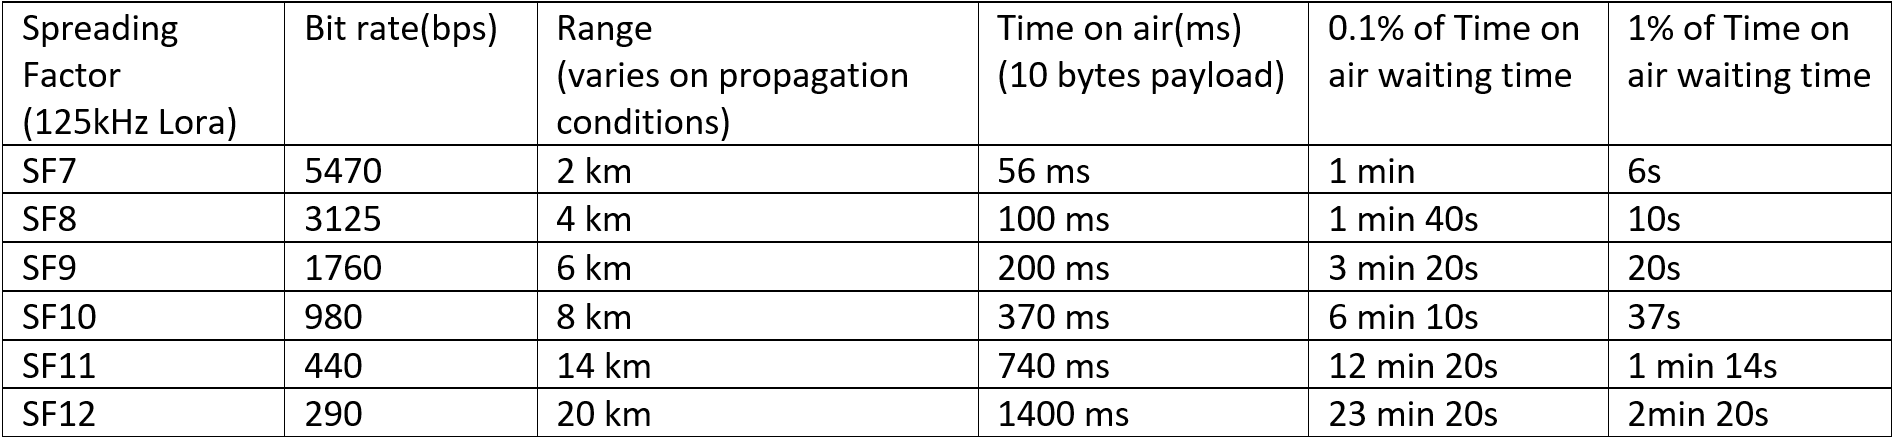
\includegraphics[width=1\textwidth]{spreading_factor_lorawan_2017-07-29}
    \caption{LoRa spread factor options \cite{24}}
    \label{fig:loraSF}
\end{figure}

This technology is very attractive for its long range capability and easy to connect nodes. It's complicated to build a full-capacity gateway which is capable of receiving packets at all frequency channels and SF in parallel. The transceiver for this application costs about \$130. Although it's also possible to build single-channel gateway which is way too cheaper, but it can receive packets at only one frequency channel and SF at once \cite{17} \cite{18} \cite{19} \cite{20} \cite{21} \cite{22} \cite{23} \cite{24}.


\section{Sigfox}
This technology focuses on short message and long range communication applications \cite{25} \cite{26}.


\section{Z-Wawe}
Z-Wave is intended for wireless connectivity for all possible smart home products, controlled by PC, phone, voice, etc. It's based on mesh network topology so every non-battery powered device works as a router to enhance the network range so the more devices are connected in one network, the stronger the network is \cite{27} \cite{28}.


\section{Thread}
This technology based on IPv6 was developed for home network controlled by smartphone, tablet or PC \cite{29} \cite{30} \cite{31}.


\section{RPMA}
The "Random Phase Multiple Access" developed by Ingenu designed for M2M and IoT applications \cite{32} \cite{rpma_ublox} \cite{34}. \textit{"RPMA has been deployed for the Machine Network, but can also be rolled out as a private network installation. It is highly suitable for regions, where the rollout of 3GPP LPWA technologies is lagging, where cellular coverage is generally weak, or where users would like to exert full control over their network deployments."}\cite{rpma_ublox}




%%%%%%%%%%%%%%%%%%%%%%%%
\part{Practical part}

\chapter{Stanovení požadavků návrhu zařízení}


Účelem tohoto projektu je rozšířit přístupový systém firmy IMA o IoT, aby bylo možné snímat veličiny jako je teplota, vlhkost, atd. bezdrátovými senzory rozmístěnými po budově.
Práce tedy zahrnuje návrh, realizace a otestování gatewaye, která shromažďuje data z bezdrátových koncových zařízení a přeposílá je na control panel přístupového systému. 
Předpokládá se, že koncová zařízení jsou senzory nebo aktuátory napájeny z baterie, tudíž pro jejich dlouhodobou životnost je kladen důraz na nízkou spotřebu vybrané bezdrátové technologie.

% \begin{figure}[!h]
%     \centering
%     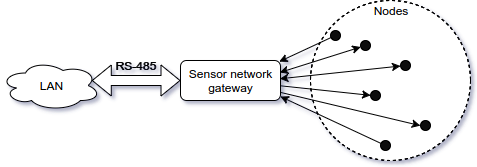
\includegraphics[width=1\textwidth]{01}
%     \caption{Blokový diagram funkce gatewaye}
%     \label{fig:block diagram of the system}
% \end{figure}


\section{Přístupové systémy}
Přístupové systémy jsou elektronické systémy řídící skrze síť přístup uživatelů do budov či objektů na základě ověření jejich identity \cite{accessControlSystem_eiprocus}.
V obrázku \ref{fig:Access control system architecture} je znázorněn příklad infrastruktury přístupového systému.

\begin{figure}[!h]
    \centering
    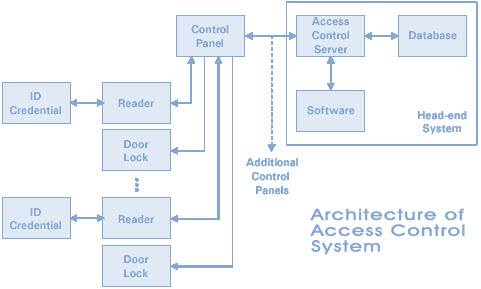
\includegraphics[width=1\textwidth]{Architetcture-of-Access-Control-System}
    \caption{Příklad architektury přístupového systému \cite{accessControlSystem_eiprocus}}
    \label{fig:Access control system architecture}
\end{figure}

ID Credential je identifikátor uživatele, např. RFID tag, otisk prstu, QR kód atd.
Reader slouží k sejmutí dat identifikátoru uživatele a odeslání do control panelu
Door lock slouží k ovládání přístupu uživatele do objektu.
Control panel vytváří rozhranní mezi access control systémem a dvojcemi readerů a door locků. 
Obvykle vytváří síť například poRS485, kde jsou zapojeny jednotky až desítky těchto dvojíc. 
V jednom systému může být jeden nebo více control panelů vytvářejících síť o jedné nebo více dvojicích reader a door lock.
Control panel komunikuje s access control systémem například přes ethernet na bázi protokolu TCP/IP.
Databáze obsahuje uživatelská ID.
Na access control serveru je spuštěn software umožňující spravování databáze a komunikaci se všemi control panely systému.
Prokáže-li se uživatel pomocí ID credential readeru, reader sejme ID uživatele a odešle na control panel, který jej následně přepošle na access control server.
Software access control vyhledá přijaté user ID v databázi a je-li nalezeno, pošle na odpovídající control panel příkaz k sepnutí odpovídajícího door locku.



\section{Implementace IoT do přístupového systému firmy IMA}
\label{sec:Implementace IoT do přístupového systému firmy IMA}
V infrastruktuře přístupového systému v obr. \ref{fig:Access control system architecture} je reader nahrazen gatewayí a ID credential bezdrátovým senzorem. 
Gateway pak komunikuje s control panelem přes rozhranní RS485 s proprietárním síťovým protokolem navrženým ve firmě IMA. 
Stávajcí přístupový systém je navržen tak, že po spuštění připojeného readeru je mu ze serveru předán seznám offline RFID karet. 
Pro gateway to je seznam adres koncových zařízení senzorové sítě. 
V případě, že uživatel přiloží ID credential odpovídající některému ze seznamu offline karet, reader přepošle příkaz "průchod".
Ekvivalentně to platí pro gateway. 
V případě že gateway přijme packet od koncového zařízení s daty ze senzorů a adresa koncového zařízení je obsažena v seznamu adres koncových zařízení,
gateway odešle příkaz "průchod" obsahující adresu koncového zařízení a data koncového zařízení.
Problém je ale v tom, že příkaz "průchod" má kapacitu na data koncového zařízení pouze 6 bytů.
Rošiřování vlastností tohoto protokolu by znamenalo mnoho komplikací, 
cílem je tedy implementace gatewaye tak, aniž by bylo nutné protokol rozšiřovat.


% - popiste infrastrukturu pristupovych systemu (obrazek a popis jednotlivych bloku), a jednak jejich vyuziti, 
% zda se pouzivaji i na neco jineho - opet clanky, ten obr. 3.1 neni dostatecny pro clanek. Mam na mysli toto:
% https://www.elprocus.com/understanding-about-types-of-access-control-systems/
% https://en.wikipedia.org/wiki/Access_control#Access_control_system_topologies

\chapter{Realizace zařízení}

\section{Výběr přenosové technologie}
Pro implementaci LPWSN je použita RF technologie LoRa se standardizovaným síťovým protokolem LoRaWAN, ale s požitím pouze jednoho kanálu.
Tento způsob řešení se liší od standardu omezením na pouze jeden kanál a SF vysílání.
Jedenokanálové řešení bylo zvoleno z toho důvodu, že plnohodnotný LoRa transceiver, který přijímá na všech osmi kanálech je příliš drahý (přibližně desetinásobná cena) a složitý k implementaci, zatímco v tomto projektu je kladen důraz na cenu a jednoduchost řešení.

Vybraná technologie používá topologii typu hvězda, tedy koncová zařízení komunikují přímo s gatewayí, 
zbytek času mohou být ve stavu nízké spotřeby, což má pozitivní vliv na životnost baterie.
Koncová zařízení od různých výrobců jsou plně kompatibilní s cizí gatewayí, tudíž není problém je implementovat do tohoto systému. 
Je pouze třeba je překonfigurovat pro vysílání na jednom použitém kanále a SF.

% tahle section by mozna mohla byt nekde jinde
% \subsection{Zabezpečení protokolu LoRaWAN}
% Protokol LoRaWAN používá AES-128 na 2 způsoby, pro síťové a aplikační zabezpečení. Jsou zde tedy 2 šifrovací klíče, NwkSKey a AppSKey.

% \subsubsection{Síťové zabezpečení}
% Síťové zabezpečení je zde aby bylo hackerům zabráněno odesílání duplikovaných paketů nebo vytváření a vysílání paketů s nasimulovanými daty.
% Poslední 4 byty paketu obsahují MIC (Message Integrity Code), který je získán zašifrováním dat síťovým klíčem NwkSKey obsahujících mimo jiné celý payload paketu (včetně paket counter). Toto umožňuje odhalit jakoukoliv manipulaci s daty v paketu. LoRaWAN paket také obsahuje counter počítající od nuly od doby kdy bylo LoRaWAN zařízení spuštěno. Toto umožňuje odhalit duplikování paketů.

% \subsubsection{Aplikační zabezpečení}
% Aplikační klíč AppSKey (Application Session Key) je použit pro zašifrování dat aplikační zprávy (App message) \cite{lwSpec} \cite{lwSecur}.


%%%%%%%%%%%%%%%%%%%%%%%%%%%%%%%%%%%%%%%%%%%%%%%%%%%%%%%%%%%%%%%%%%%%%%%%%%
\section{Výběr komponent}
\subsection{Microcontroller}
Pro toto zařízení je zvolen mikrocontroller STM32L073RZ se zaměřením na nízkou spotřebu, jelikož je levný, má dostačující vlastnosti a je dostupný ve formě vývojového kitu NUCLEO-L073RZ který byl použit pro  vývoj zařízení. Mezi hlavní vlastnosti patří \cite{nucleoST}:
\begin{itemize}    
    \item {Architektura ARM Cortex-M0+ 32-bit RISC}
    \item{Interní Flash paměť 192 KB}
    \item{Interní SRAM paměť 20 KB}
    \item{Interní EEPROM paměť 6 KB}
    \item {Až 32 MHz CPU}
    \item {2X SPI, 3x I2C, 4x USART, LIN, ADC}
\end{itemize}

Pořizovací cena kitu přímo na stránce výrobce www.st.com je \$13 \cite{nucleoST} \cite{nucleoMbed}.
\begin{figure}[!h]
    \centering
    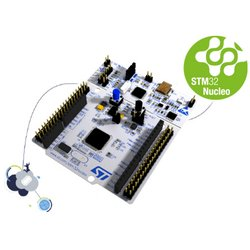
\includegraphics[width=0.4\textwidth]{Nucleo64}
    \caption{Vývojový kit NUCLEO-L073RZ \cite{nucleoST}}
    \label{fig:02}
\end{figure}

\subsection{LoRa transceiver}
Lora transceiver čip doposud vyrábí pouze Semtech, pro použití v Evropském pásmu je určen typ SX1276.
V tomto návrhu je použita deska RFM95w od firmy HopeRF s integrovaným čipem SX1276 \cite{RFM95w}.
Pro vývoj zařízení byl využit tento transciever v tzv. Dragino LoRa Shield \cite{draginoWiki}, který má stejně jako použitý vývojový kit, pinout kompatibilní s Arduino UNO. Pořizovací cena samotného transceiveru RFM95w je okolo \$7, cena Dragino Shieldu se pohybuje okolo \$22 na ebay.

\begin{figure}[!h]
    \centering
    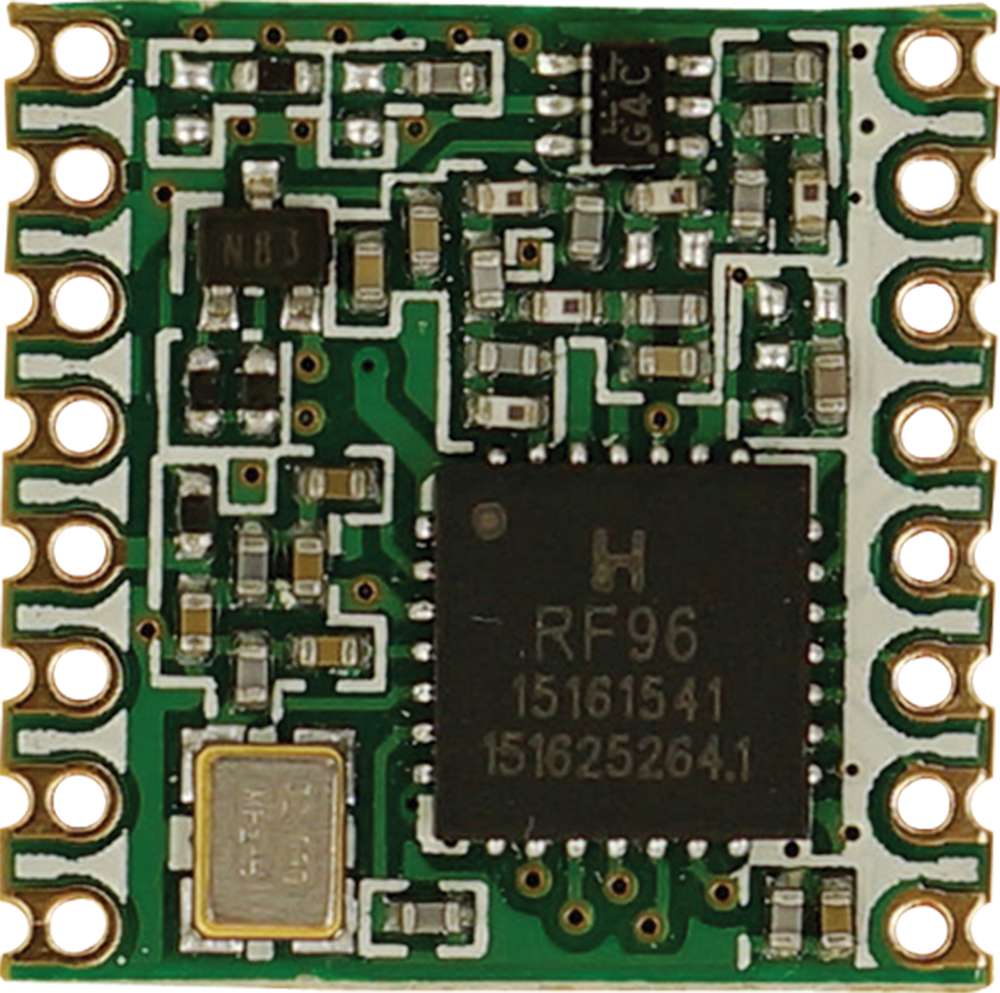
\includegraphics[width=0.2\textwidth]{RFM95w}
    \caption{LoRa transceiver RFM95w \cite{RFM95w}}
    \label{fig:02}
\end{figure}

\subsection{RS485 transceiver}
SparkFun Transceiver Breakout - RS485 převádí rozhranní UART na RS485, pří vstupním napětí 3.3 V. A je dostupný za cenu okolo \$10 \cite{rs485tr}.

\begin{figure}[!h]
    \centering
    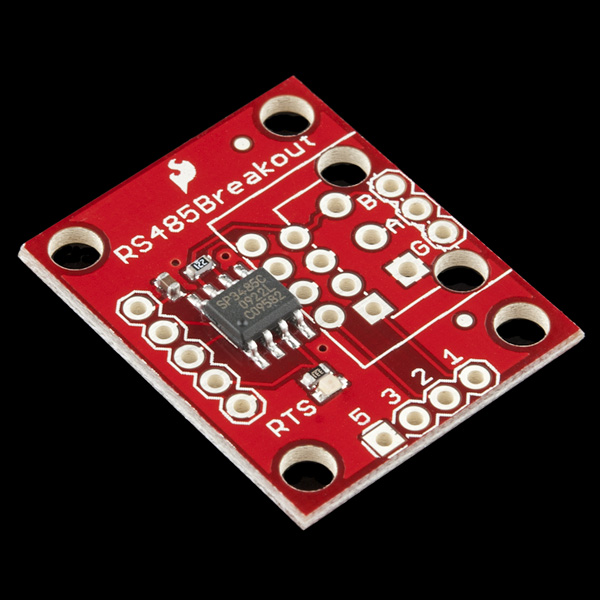
\includegraphics[width=0.4\textwidth]{rs485transceiver}
    \caption{RS485 transceiver \cite{rs485tr}}
    \label{fig:rs485transceiver}
\end{figure}

\newpage
%%%%%%%%%%%%%%%%%%%%%%%%%%%%%%%%%%%%%%%%%%%%%%%%%%%%%%%%%%%%%%%%%%%%%%%%%
\section{Implementace LoRaWAN sítě}
Jednokanálové použití technologie LoRa umožňuje použít transceiver navržený pro koncová zařízení, 
kterým jsou pakety kontinuálně odposlouchávány na jednom nastaveném kanále a SF. 
Tyto dva parametry jsou nakonfigurovány na všech zařízeních v síti stejně.

Jak je popsáno v sekci \ref{sec:Implementace IoT do přístupového systému firmy IMA}, 
použitý protokol pro komunikaci s control panelem přístupového systému firmy IMA zajišťuje posílání dat z koncových zařízení příkazem "průchod", 
který má kapacitu na data z koncového zařízení pouze 6 B. 
Systém je proto navržen neobvyklým způsobem. 
Přijme-li gateway LoRaWAN paket, nejprve zkontroluje zda zná adresu zařízení, pokud ano, přečte z paměti i typ zařízení,
 paket dešifruje a dekóduje payload, čímž získá konečné hodnoty senzorů, které pak dále pošle přes RS485 rozhraní na zařízení typu master.

LoRaWAN device address a typ každého zařízení v síti je uložena v EEPROM (non-volatile) paměti gatewaye a jsou nastavována na z access control serveru.
Všechna zařízení v síti mají nastavené stejné šifrovací klíče a gateway je má uložené v EEPROM.

Pro tento projekt byla vyvinuta knihovna pro dekódování payloadu na základě dokumentů \cite{lwSpec} \cite{lwSecur}.


%%%%%%%%%%%%%%%%%%%%%%%%%%%%%%%%%%%%%%%%%%%%%%%%%%%%%%%%%%%%%%%%%%%%%%%%%%
\section{Implementace komunkičního protokolu v síti IMA\_RS485 pro komunikaci s control panelem}
V tomto projektu je komunikace protokolu IMA\_RS485 naprogramována v souborech rs485\_protocol.h a rs485\_protocol.c. 
Jedná se o kolizní protokol v síti, kde je připojen jedno zařízení typu master, a jeden nebo více zařízení v typu slave.

\begin{table}[!h]
    \centering
    \begin{tabular}{ |c|c| }
     \hline

     Baud rate              & 9600           \\ \hline
     Data bits              & 8                 \\ \hline
     Parity                 & none              \\ \hline
     Stop bits              & 1                 \\ \hline

    \end{tabular}
    \caption{Fyzické vlastnosti IMA\_RS485 sítě}
    \label{table:3}
\end{table}

\newpage
\subsection{Syntaxe příkazů}
Komunikace v síti probíhá formou příkazů, které mají specifikovanou syntaxi v tabulce \ref{table:syntaxePrikazu}.

\begin{table}[!h]
    \centering
\begin{tabular}{ |c|| p{1.5cm} | p{1.5cm} | p{1cm} | p{1cm} | p{1cm} | p{1cm} | }
 \hline
 popis      & adresa příjemce & adresa odesílatele & typ příkazu & délka dat & data & crc\\ \hline
 počet bytů & 1               & 1   & 1     & 2     & délka dat     & 1 \\ 
 \hline
\end{tabular}
    \caption{Syntaxe příkazu pro komunikaci v síti IMA\_RS485}
    \label{table:syntaxePrikazu}
\end{table}

Typy příkazu jsou zadefinované konstanty s předponou CKP\_CMD\_ v souboru ./Inc/rs485\_protocol.h.
Příkazy odeslané zařízením typu master obsahují navíc synchronizační byte na začátku 0xAA.
CRC je pro kontrolu XOR přes všechny předchozí byty v celém příkazu kromě synchronizačního bytu.

\subsection{Adresace zařízení v síti}
Každé zařízení na této sběrnici má svoji adresu, která mu je nastavena externě. Zařízení typu master má adresu  0xFF, adresa pro všechny (broadcast) je 0x00 a zařízení v této sítí můžou mít adresu libovolnou (krom těchto dvou) nesmí zde však být připojena 2 zařízení s nastavenou stejnou adresou.

\subsection{Statusy}
Zařízení typu slave má dva možné statusy v síti IMA\_RS485, offline a online. Zařízení typu slave má povoleno odesílat příkaz "průchod" pouze má-li status online.  
Zařízení typu slave odesílá příkaz obsahující informaci o jeho statusu periodicky s typem příkazu 0x10 a jedním bytem dat označujícím status. 
Pro status online je tento byte 0x00 a pro status offline 0xEE. 
Tento příkaz je odesílán s intervalem 10 s, pokud zařízení má status offline a s intervalem 30 s, pokud má zařízení status online.
Status zařízení mění pouze zařízení typu master odesláním příkazu s typem 0x41 pro přepnutí na status online a 0x42 pro přepnutí na status offline.
Zařízení typu slave svůj status přepne samo pouze v případě, že má status online a zařízení typu master přestane odpovídat na příkaz průchod, jak je popsáno v sekci \ref{sec:Odesílání dat z koncových zařízení}.
Je-li zařízení spuštěno, je ve stavu offline a jelikož nemá povoleno odesílat příkaz "průchod", přijatá data z koncových zařízení jsou zahazována. 
Zařízení typu slave pouze odpovídá na příkazy od zařízení typu master a čeká na příkaz od zařízení typu master k přepnutí na status online.


\subsection{Přidávání LoRaWAN zařízení do systému}
Pokud zařízení typu master přijme příkaz od zařízení typu slave oznamující že je ve stavu offline, nejprve tomuto zařízení pošle seznam LoRaWAN adres všech známých koncových zařízení a následně toto zařízení přepne do stavu online.
Přijímání seznamu adres je realizováno sekvencí příkazů typu 0x8F. 

Níže v tabulce \ref{table:2} je příklad sekvence příkazů odesílaných mezi zařízením typu masterem a zařízením typu slavem během předávání seznamu LoRaWAN device address koncových zařízení, kde zařízení typu slave má adresu 0x10 a zařízení typu master standardně 0xFF. Jak již bylo řečeno, příkazy od zařízení typu master lze jednoduše odlišit tím, že vždy začínají bytem 0xAA.


\begin{table}[!h]
    \begin{tabular}{ |l|p{10cm}| }
    \hline
    příkaz      &  data    \\ \hline \hline
    master: start      &  AA 10 FF 8F 02 00 00 00 62    \\ \hline
    slave: ACK        &  FF 10 06 02 00 8F 00 64    \\ \hline
    master: data     &  AA 10 FF 8F 21 00 01 B1 C4 12 00 00 00 00 00 B2 C4 12 00 00 00 00 00 B3 C4 12 00 00 00 00 00 B4 C4 12 00 00 00 00 00 44 \\ \hline
    slave: ACK      &  FF 10 06 02 00 8F 01 65   \\ \hline
    master: data     &  AA 10 FF 8F 19 00 02 B5 C4 12 00 00 00 00 00 B6 C4 12 00 00 00 00 00 F6 1F 01 26 00 00 00 00 B6 \\ \hline
    slave: ACK      &   FF 10 06 02 00 8F 02 66   \\ \hline
    master: konec   &   AA 10 FF 8F 04 00 03 FF 2A 57 E5   \\ \hline
    slave: ACK      &   FF 10 06 02 00 8F 03 67  \\ \hline
    \end{tabular}
    \caption{Příklad sekvence příkazů odesílaných mezi zařízením typu master a zařízením typu slave během předávání seznamu LoRaWAN device address koncových zařízení}
    \label{table:2}
\end{table}

LoraWAN protokol používá 4-bytové adresy koncových zařízení.
Adresy předávány touto sekvencí jsou dlouhé 8-bytové. První 4 byty je tedy LoRaWAN device address, pátý byte je typ zařízení a zbylé 3 byty jsou nevyužity, jejich použití je možné v případě změn či rozšiřování vlastností systému. 

První Byte dat je counter paketu začínající od nuly, který označuje číslo odeslaného paketu v sekvenci. Na každý tento paket v sekvenci zařízení typu slave odpovídá ACK příkaz, který se liší od obyčejného ACK příkazu tím, že v datech paketu navíc obsahuje counter pakety v sekvenci.
První příkaz této sekvence má délku dat 2 byty, které mají hodnotu 0x00 přičemž první je counter.
Další příkazy hned za counter bytem obsahují několik osmibytových adres, jejichž počet je různý.
Příkaz ukončující tuto sekvenci příkazů má délku 4 byty, což je tedy counter, 0xFF a 2 byty CRC přes všechny odeslané adresy (nepodstatné, tudíž ho nepoužívám).

\subsection{Odesílání dat z koncových zařízení}
\label{sec:Odesílání dat z koncových zařízení}
Jak je popsáno v sekci \ref{sec:Implementace IoT do přístupového systému firmy IMA}, tudíž data z koncových zařízení jsou odesílána příkazem "průchod", jehož typ je 0x10 a kapacita na data z koncového zařízení je pouze 6 B. 
První byte dat označuje typ průchodu, byl zvolen konstantní byte 0xD0. Dále následuje LoRaWAN adresa koncového zařízení od kterého byl paket přijat. Dále následují 4 byty dat ze senzoru, další 2 byty signalizující čas průchodu, což v tomto projektu není použito a tyto dva byty mají vždy hodnotu 0xFF. A nakonec jsou další 2 byty obsahující data ze senzoru.

Příklad příkazu: FF 1F 10 0D 00 D0 F6 1F 01 29 AD 0A 5A 27 FF FF DE 09 E1.

Data příkazu jsou níže rozepsána v tabulce \ref{table:prikladprikazpruchod}.

\begin{table}[!h]
    \centering
\begin{tabular}{ | p{1.5cm} | p{3cm} | p{2.5cm} | p{1.3cm} | p{1.3cm} |  }
 \hline
 typ průchodu & LoRaWAN device address & data (4B)     & cas   & data (2B) \\ \hline
 D0           & F6 1F 01 29            &  AD 0A 5A 27  & FF FF & DE 09     \\ 
 \hline
\end{tabular}
    \caption{Příklad dat příkazu "průchod" odeslaného z gatewaye na zarizeni typu master, obsahující data z koncových zařízení}
    \label{table:prikladprikazpruchod}
\end{table}

Zařízení typu master na příkaz "průchod" odpovídá příkazem ACK. Zařízení typu slave na tuto odpověď čeká standardně 3 sekundy, ale tento parametr je nastavitelný. Pokud v tomto timeoutu zařízení typu master neodpoví, zařízení typu slave příkaz "průchod" zopakuje přičemž změní typ příkazu na 0x20. Pokud zařízení typu master ani na třetí opakování neodpoví ACK, zařízení typu slave se přepne do stavu offline a vymaže frontu příkazů "průchod" k odeslání.

\subsection{Potvrzení}
Zařízení typu slave odpovídá na každý příkaz od zařízení typu master ACK. Typ příkazu ACK je 0x06 a data příkazu obsahují jeden byte signalizující typ příkazu na který je právě odpovídáno potvrzením.
Zařízení typu master odpovídá ACK se stejným typem příkazu 0x06, ale s žádnými daty příkazu.

\subsection{Dotaz na příznaky}
Zařízení typu master se může zeptat s jak dlouhými adresami zařízení typu slave pracuje s typem příkazu 0x49. Zařízení typu slave na to odpovídá ACK s tím, že v datech příkazu je navíc byte 0x04. Zařízení typu master pak počítá s tím, že zařízení typu slave pracuje se 64-bit adresami (ve skutečnosti ale používá 32-bitové a zbylé 4 byty v příkazu průchod jsou pro data z koncového zařízení).

%%%%%%%%%%%%%%%%%%%%%%%%%%%%%%%%%%%%%%%%%%%%%%%%%%%%%%
\section{Komunikace přes USB}
Gateway má implementovanou komunikaci přes USB, což má za účel konfiguraci systému a logování. K přípojení přes USB lze použít PC s  aplikací terminálu s nastavením viz tabulka \ref{table:usb_term}.

\begin{table}[!h]
    \centering
    \begin{tabular}{ |c|c| }
     \hline

     Baud rate              & 115200           \\ \hline
     Data bits              & 8                 \\ \hline
     Parity                 & none              \\ \hline
     Stop bits              & 1                 \\ \hline
     Flow control           & none               \\ \hline

    \end{tabular}
    \caption{Nastavení USB terminálu}
    \label{table:usb_term}
\end{table}

Při komunikaci jsou data standardně oddělována bytem CR (carriage return) 0x0D, ale je akceptována i sekvence CR LF (Line Feed), tedy 0x0D 0x0A. 

%%%%%%%%%%%%%%%%%%%%%%%%%%
\subsection{Log aplikace}
Gateway loguje informace o proběhlých událostech přes USB. 
Níže je příklad výpisu dat pro případ, že gateway přjala LoRaWAN paket z koncového zařízení v síti.

Nejprve jsou vypsána data týkající se LoRaWAN protokolu, zašifrovaný i dešifrovaný payload, typ zařízení a konečné informace dekódované z payloadu.
Řádek začínajci předponou "Tx -> RS-485:" obsahuje data odeslané k zařízení typu master přes RS485 síť a následující řádek začínající předponou "Rx -> RS-485:" obsahuje odpověď od zařízení typu master.

\begin{lstlisting}
______________________________________________________
Rx -> LoRaWAN, pktCntr: 6
RSSI: -51, SNR: 9, length: 22

Message type: Unconfirmed Data Up
Packet rawData: "40F61F0128C0D62508D970CB071595D115BAC68F6663"
Device Address: "F61F0128"
FCnt: 9686
message (encrypted): "D970CB071595D115BA"
MHDR: 40; FCtrl: C0; FPort: 08; MIC: "C68F6663"
adaptive data rate: true; ack: false
message HEX (decrypted): "013566779600FFFFAF"

Sensor type: RHF1S001
temperature: 23.30 C, humidity: 52 %
period: 300 s, RSSI: -51 dBm, SNR: 9 dB, battery voltage: 3.2 V
Tx -> RS-485: "FF1F100D00D0F61F01281A0934CDFFFF09202E"
______________________________________________________
Rx -> RS-485: "AA1FFF060000E6"
ACK
\end{lstlisting}

%%%%%%%%%%%%%%%%%%%%%%%%%%
\subsection{Konfigurace systému}
\label{sec:konfigurace}
Konfigurace gatewaye se provádí opět přes USB port. Je do ní vstoupeno odesláním příkazu
"config", následuje vypsání současného stavu konfigurace a dále je vypsáno konfigurační menu, kde uživatel vybere jednotlivý bod menu zadáním jeho čísla na začátku řádku.
Níže je zobrazen příklad výpisu po vstupu do konfigurace.

\begin{lstlisting}
    _________________Entering configuration setup________________
    
    System configuration:
    
    *** LoRa channel: 
    channel: 0 (868.1 Mhz)
    SF7
    
    *** RS485 channel: 
    my address: 10
    master address: FF
    timeout: 3 s
    
    *** LoRaWAN keys: 
    NwSKey:  FD 90 0D 8C 70 9F 19 24 18 EC FD D4 28 0C AC 47
    AppSKey:  68 9F D0 AC 7A 0F 95 58 B1 19 A0 16 17 F4 16 33
    
    
    Config menu:
    1 -> Config LoRa channel
    2 -> Config RS485 channel
    3 -> Config LoRaWAN protocol
    4 -> Print all LoRaWAN devices
    5 -> Erase all LoRaWAN devices
    6 -> Restore to default configuration
    7 -> Exit without save
    8 -> Save and exit
\end{lstlisting}
    

Z konfigurace je možné vystoupit kdykoliv bez uložení změn příkazem "quit". 
Při vstoupení do konfigurace je pozastavena činnost gatewaye, komunikace s koncovými zařízeními LoRaWAN síťě a komunikace se zařízením typu master v síti RS485 nejsou aktivní.
Jsou zde tedy 3 stavy konfigurace, přičemž je možné vždy jednotlivá nastavení přeskakovat odesláním "prázdného příkazu" 0x0D (v terminálu obvykle stačí stisknout Enter). Systém při konfiguraci vždy vypíše jaká data mají být zadána v jakém tvaru a zároveň současnou hodnotu měněného parametru. Zadaná data uživatelem jsou vždy zkontrolována zda splňují požadovaný tvar. Pokud ne, uživatel je o tom informován a vyzván k dalšímu pokusu.
Po provedení konfigurace následuje vždy návrat zpět do hlavního menu. Pro uložení nové konfigurace je potřeba v menu vybrat "Save and exit", gateway pak následně vypíše které parametry byly změněny a provede restart.

\subsubsection{Config LoRa channel}
Konfigurace LoRa RF kanálu zahrnuje nastavení SF a frekvenční pásmo. Níže je příklad konfigurace.

\begin{lstlisting}
LoRa channel configuration:
Enter SF number (7-12)
(current: 7)
8
SF8 set.

Enter LoRa channel number (0-7)
ch0 is 868.1 Mhz
ch1 is 868.3 Mhz
ch2 is 868.5 Mhz
ch3 is 867.1 Mhz
ch4 is 867.3 Mhz
ch5 is 867.5 Mhz
ch6 is 867.7 Mhz
ch7 is 869.0 Mhz
(current: 0)
1
channel 1 set.
\end{lstlisting}

\subsubsection{Config RS485 channel}
Konfigurace RS485 kanálu pro komunikaci se zařízením typu master zahrnuje nastavení adresy tohoto zařízení, adresa zařízení typu master a timeout, což je doba čekání na potvrzení od zařízení typu master po odeslání příkazu "průchod". Níže je příklad konfigurace.

\begin{lstlisting}
RS485 channel configuration:
Enter address of this device, FF and 00 are reserved.
(current: 10)
11
Address of this device is set to: 11

Enter master address: 
(current: FF)
FE
Master address is set to: FE

Enter timeout (seconds)
(current: 3)
5
timeout set to: 5 s
\end{lstlisting}


\subsubsection{Config LoRaWAN protocol}
Konfigurace LoRaWAN protokolu zahrnuje nastavení šifrovacích klíčů NwkSKey a AppSKey. Níže je příklad konfigurace.

\begin{lstlisting}
LoRaWAN protocol configuration:
Enter NwkSKey (16 bytes in HEX)
(current:  FD 90 0D 8C 70 9F 19 24 18 EC FD D4 28 0C AC 47)
11111111222222223333333344444444
NwSKey set to: 11 11 11 11 22 22 22 22 33 33 33 33 44 44 44 44

Enter AppSKey (16 bytes in HEX)
(current:  68 9F D0 AC 7A 0F 95 58 B1 19 A0 16 17 F4 16 33)
11111111222222223333333344444444
AppSKey set to: 11 11 11 11 22 22 22 22 33 33 33 33 44 44 44 44
\end{lstlisting}


\subsubsection{Print all LoRaWAN devices}
Vypíše všechna LoRaWAN zařízení uložená v paměti. Níže je příklad.


\begin{lstlisting}
number.......................0:
Device Address:  B1 C4 12 00
Device Type: RH1S001
number.......................1:
Device Address:  B2 C4 12 00
Device Type: RH1S001
number.......................2:
Device Address:  B3 C4 12 00
Device Type: RH1S001
number.......................3:
Device Address:  B4 C4 12 00
Device Type: IMA_tempPress
number.......................4:
Device Address:  B5 C4 12 00
Device Type: IMA_tempPress
\end{lstlisting}



\subsubsection{Restore default configuration}
Po zvolení této možnosti je načtena defaultní konfigurace systému, která obsahuje hodnoty viz tabulka \ref{table:5}. Tyto defaultní hodnoty jsou nastaveny v programu a slouží především pro testovací účely.

\begin{table}[!h]
    \centering
    \begin{tabular}{ |l|l| }
     \hline

     popis              & hodnota         \\ \hline \hline
     RS485 myAddr       & 0x10            \\ \hline
     RS485 MasterAddr   & 0xFF            \\ \hline
     RS485 timeout      & 3               \\ \hline
     LoRa SF            & SF7             \\ \hline
     LoRa channel       & 0 (868.1 Mhz)   \\ \hline
     NwSKey             & FD 90 0D 8C 70 9F 19 24 18 EC FD D4 28 0C AC 47  \\ \hline
     AppSKey            & 68 9F D0 AC 7A 0F 95 58 B1 19 A0 16 17 F4 16 33  \\ \hline

    \end{tabular}
    \caption{Defaultní konfigurace systému}
    \label{table:5}
\end{table}


\newpage
%%%%%%%%%%%%%%%%%%%%%%%%%%%%%%%%%%%%%%%%%%%%%%%%%%%%%%
\section{Koncová zařízení}
Jelikož používaný protokol ke komunikaci se zařízením typu master je omezen na pouhých 6 B na jeden paket, payload koncových zařízení je dekódován v gatewayi a v paketu odeslaném na zařízení typu master jsou pouze vybraná nejdůležitější data, která se vejdou do této velikosti.
Prote společně s LoRaWAN device address koncového zařízení je v gatewayi uložen i typ zařízení zadefinován jedním bytem a na základě typu zařízení gateway rozpozná jak dekódovat payload.

Momentálně jsou podporovány dva typy koncových zařízení, dle potřeby je možné rozšířit FW gatewaye o další typy koncových zařízení.

\begin{table}[!h]
    \centering
    \begin{tabular}{ |l|l| }
     \hline

     Typ zařízení       & Hodnota         \\ \hline \hline
     RHF1S001           & 0x00            \\ \hline
     IMA\_tempPress     & 0x01            \\ \hline
     
    \end{tabular}
    \caption{Typy koncových zařízení}
    \label{table:TypyKoncZarizeni}
\end{table}

\subsection{Zpracování dat jednotlivých typů koncových zařízení}
Níže je popsáno pro jednotlivá podporovaná koncová zařízení jak jsou data uložena v datové struktuře, jak jsou data z této struktury zpracována a zobrazena a nakonec jak vybraná data jsou zapsána do výsledného bufferu o délce 6 B, který je odeslán na zařízení typu master příkazem "průchod".

\subsubsection{RHF1S001}
Senzor od firmy RisingHF měří teplotu a vlhkost.

\begin{lstlisting}[style=CStyle]
    /* RHF1S001 data structure */   
    typedef struct {
        int16_t temperature;
        uint8_t humidity;
        uint16_t period;
        int8_t rssi;
        int8_t snr;
        uint8_t battery;
    } RHF1S001_data_t;

    /* Print the data from the structure */
    printf("temperature: %d.%d C, ", RHF1S001_data.temperature / 100, RHF1S001_data.temperature % 100);
    printf("humidity: %d %%\n", RHF1S001_data.humidity);
    printf("period: %d s, ", (int)RHF1S001_data.period);
    printf("RSSI: %d dBm, ", RHF1S001_data.rssi);
    printf("SNR: %d dB, ", RHF1S001_data.snr);
    printf("battery voltage: %d.%d V\r\n", RHF1S001_data.battery/10, RHF1S001_data.battery % 10);

    /* Put the data into 6B long buffer, that is transmitted to the master */
    buffer[0] = RHF1S001_data.temperature & 0xFF;
    buffer[1] = RHF1S001_data.temperature >> 8;
    buffer[2] = RHF1S001_data.humidity;
    buffer[3] = RHF1S001_data.rssi;
    buffer[4] = RHF1S001_data.snr;
    buffer[5] = RHF1S001_data.battery;
\end{lstlisting}


\subsubsection{IMA\_tempPress}
Senzor vytvořený ve firmě IMA, měřící teplotu a tlak.

\begin{lstlisting}[style=CStyle]
    /* IMA_tempPress data structure */   
    typedef struct {
        int16_t temperature;
        uint16_t pressure;
        int8_t rssi;
        int8_t snr;
    } IMA_tempPress_data_t;
    
    /* print the data from the structure */
    printf("temperature: %d.%d C, ", IMA_tempPress_data.temperature / 100, IMA_tempPress_data.temperature % 100);
    printf("pressure: %d.%d Pa\r\n", IMA_tempPress_data.pressure/10, IMA_tempPress_data.pressure % 10);
    printf("RSSI: %d dBm, SNR: %d dB\r\n", IMA_tempPress_data.rssi, IMA_tempPress_data.snr);

    /* Put the data into 6B long buffer, that is transmitted to the K4 server */
    buffer[0] = IMA_tempPress_data.temperature & 0xFF;
    buffer[1] = IMA_tempPress_data.temperature >> 8;
    buffer[2] = IMA_tempPress_data.pressure & 0xFF;
    buffer[3] = IMA_tempPress_data.pressure >> 8;
    buffer[4] = IMA_tempPress_data.rssi;
    buffer[5] = IMA_tempPress_data.snr;
\end{lstlisting}


\subsection{Přidávání koncových zařízení ze serveru K4}
Koncocová zařízení sítě se nastavují ze serveru K4 v podobě seznamu offline karet s délkou UID 8 B.
LoRaWAN device address je dlouhá 4 B, jeden byte je navíc použit pro typ koncového zařízení, zbylé 3 byty jsou nuly.
Jelikož typ zařízení je uložen v gatewayi i na K4 serveru. Při odesílání příkazu průchod se tedy už typ zařízení neposílá z důvodu datového omezení tohoto příkazu.
Na serveru K4 se UID nastavuje jako dekadické číslo.
Níže je příklad vytvoření výsledného čísla obsahující DevAddr a typ zařízení, které se zadává do K4 serveru.

\subsubsection{Příklad}
Pro případ, kde typ zařízení je 01 a DevAddr AABBCCDD (little endian) výsledné číslo v hexadecimální podobě je 01DDCCBBAA. Následně se překládá do decimalni podoby, výsledné číslo k zadání do K4 serveru je tedy 8016149418.


%%%%%%%%%%%%%%%%%%%%%%%%%%%%%%%%%%%%%%%%%%%%%%%%%%%%%%
\section{Využití non-volatile paměťi gatewaye}
Konfigurace a adresy s typy všech koncových zařízení v LoRaWAN síti jsou uloženy v non-volatile paměti EEPROM gatewaye o kapacitě 6144 B. 
Paměť je tedy rozdělená tak, že od adresy 0 až po 6080 je prostor pro ukládání LoRaWAN zařízení a od 6080 až po 6144 je prostor pro ukládání konfigurace gatewaye.

Každé LoRaWan zařízení v síti má v paměti uložené LoRaWAN device address (4 byty), typ zařízení (1 byte) a další 3 byty jsou rezervovány. 
Jedno koncové zařízení v paměti tedy zabírá  8 B, takže gateway má kapacitu paměti pro až 760 koncových zařízení.


%%%%%%%%%%%%%%%%%%%%%%%%%%%%%%%%%%%%%%%%%%%%%%%%%%%%%%
\section{Zapojení}
LoRa shield \cite{draginoWiki} je nasazen přímo na vývojový kit Nukleo. Kit neobsahuje ISCP konektor, který je součástí pinoutu Arduino UNO a LoRa shield má SPI piny MISO a MOSI přivedeny právě na tento konektor. Musí být tedy propojeny externě viz obrázek \ref{fig:03}. Jumpery na Dragino LoRa shieldu musí také být stejně jako v obrázku.

\begin{figure}[!h]
    \centering
    \includegraphics[width=1\textwidth]{foto01}
    \caption{foto zapojení}
    \label{fig:03}
\end{figure}

Pro komunikaci s LoRa transceiverem je tedy použito SPI1, pro komunikaci přes USB je použito USART2 a pro komunikaci přes RS485 je použito UART1.

\begin{table}[h]
    \centering
    \begin{tabular}{ |c|c|c| }
     \hline

     Periférie          & Název pinu & Pin procesoru           \\ \hline \hline
     
                        & RX  &   PC1            \\
    RS485 transceiver   & TX  &   PC0       \\
                        & RTS  &  PB1      \\     \hline

                        & CS    &  PB6             \\
                        & CLK   &  PA5        \\
   LoRa transceiver     & MISO  &  PA6     \\
                        & MOSI  &  PA7        \\
                        & RST   & PC7          \\
                        & DIO0  & PA10         \\
                        \hline

    \end{tabular}
    \caption{Pinout připojení externích periférií k procesoru}
    \label{table:3}
\end{table}

%%%%%%%%%%%%%%%%%%%%%%%%%%%%%%%%%%%%%%%%%%%%%%%%
\section{Naprogramování}
K naprogramování MCU byla použita HAL knihovna a inicializační nástroj STM32CubeMX poskytnuté výrobcem, tedy ST Microelectronics.
Zdrojové soubory programu byly vyvíjeny v textovém editoru VS-Code, ke kompilaci zdrojových souborů byl použit kompilátor arm-none-eabi-gcc a jako pomocný nástroj makefile skript. 

\subsection{Zdrojové soubory projektu}
Pro šifrování LoRaWAN paketu byla použita knihovna AES-128, dostupná na githubu \cite{AESlib} a knihovna OpenPANA také dostupná z githubu \cite{CMAClib}.
Níže je seznam zdrojových souborů.

\begin{figure}[!h]
    \dirtree{%
        .1 Drivers \DTcomment{STM32 Drivers}.
        .1 Inc\DTcomment{Headers}.
            .2 aes.h\DTcomment{AES-128 library for LoRaWAN paket encryption}.
            .2 cmac.h\DTcomment{library for CMAC calculation in LoRaWAN protocol}.
            .2 LinkedList\_ByteArray.h \DTcomment{Byte array linked list library for stacks}.
            .2 LoRaWAN\_paket.h\DTcomment{LoRaWAN library for paket data decoding}.
            .2 stm32l0xx\_hal\_conf.h\DTcomment{HAL initialization of peripherals}.
            .2 ByteArray.h\DTcomment{Library for Byte array operations}.
            .2 LoRa.h\DTcomment{Library for interfacing LoRa transceiver}.
            .2 main.h\DTcomment{Main file}.
            .2 stm32l0xx\_it.h\DTcomment{HAL initialization of peripherals}.
            .2 eeprom.h\DTcomment{Library for eeprom operations}.
            .2 LoRa\_sensors.h\DTcomment{Library for decoding data from payload}.
            .2 rs485\_protocol.h\DTcomment{Library for RS485 IMA protocol}.
            .2 usb.h \DTcomment{Library for USB communication and system configuration}.
        .1 Src\DTcomment{Sources}.
            .2 aes.c \DTcomment{source file to the aes.h}.
            .2 aes.c \DTcomment{source file to the cmac.h}.
            .2 LinkedList\_ByteArray.c \DTcomment{source file to the LinkedList\_ByteArray.h}.
            .2 LoRaWAN\_paket.c  \DTcomment{source file to the LoRaWAN\_paket.h}.
            .2 stm32l0xx\_hal\_msp.c \DTcomment{HAL source file}.
            .2 ByteArray.c  \DTcomment{source file to the ByteArray.h}.
            .2 LoRa.c \DTcomment{source file to the LoRa.h}.
            .2 main.c \DTcomment{main source file}.
            .2 stm32l0xx\_it.c \DTcomment{HAL source file}.
            .2 eeprom.c \DTcomment{source file to the eeprom.h}.
            .2 LoRa\_sensors.c \DTcomment{source file to the LoRa\_sensors.h}.
            .2 rs485\_protocol.c  \DTcomment{source file to the rs485\_protocol.h}.
            .2 system\_stm32l0xx.c \DTcomment{HAL source file}.
            .2 usb.h \DTcomment{source file to the usb.h}.
    }
\end{figure}


\subsection{Nahrání programu do MCU}
Výstupem kompilace je soubor s koncovkou .binary, který je nahrán do MCU. K tomuto nahrání není potřeba žádný speciální SW nebo HW.
Stačí kit připojit k PC přes USB, v PC se kit zobrazí jako flash disk. Zkompilovaný program s koncovkou .binary stačí překopírovat na toto zařízení. 
Po dobu kopírování souboru bliká na kitu LED1 červená/zelená. Jakmile kopírování skončí, program na kitu je spuštěn, případně je možné kit resetovat černým tlačítkem reset.
Pro uvedení Gatewaye do provozu je nutné se připojit k zařízení přes USB a nastavit všechny parametry viz sekce \ref{sec:konfigurace}.  
% \chapter{Measurement Results and Discussion}
\chapter{Měření výsledky a diskuse}
%%%%%%%%%%%%%%%%%%%%%%%%%%%%%%%%%%%%%%%%%%%%%%%%%%%%%%%%%%%%%%%%%%%%%%%%%%%%%%%%%%%%%%%
One floor block of university building is selected to perform the test. It is equipped with twelve CKP devices, each controlling one Door Lock and one Reader. One Gateway is added to the infrastructure, i.e., thirteen devices are connected to one RS485 network. Two temperature/humidity sensor nodes are wirelessly connected to the Gateway. The Gateway and CKP devices are connected via RS485 network as shown in Fig. \ref{fig:Access control system architecture}. The specific location of CKP devices, Gateway and two sensor nodes on the floor is shown in Fig. \ref{fig:CorridorFloorPlan}.


The long-term operation test is carried out from 21$^{st}$ September to 31$^{th}$ October, i.e., in the period involving the presence of students and employees in the classrooms and offices on the monitored floor of the university.
During this period, the Control Panel received 1~876~978 packets (14~074~522 Bytes) and sent 1~101~556 packets (8~295~219 Bytes) from/to RS485 network. 
The lengths of all 2~978~534 packets, i.e., 22~369~741 Bytes, are recorded in RS485 network during long-term operation test and the frequency analysis  method, i.e., the number of packet lengths in monitored period, is performed. Three packets reach the largest value, i.e., 40 Bytes. 
Considering the total amount of packets, it is negligible quantity, i.e, 1.3E-04\%. However, given the nature of the system, i.e., the system with the primary function of access to a restricted area, the worst-case scenario is considered to be an uncrossable limit. 
Number of sensor nodes that can be wirelessly connected to the Gateway and does not affect the existing access control system, can be calculated in dependence on used RS485 data rate. The reserve of the data rate is considered in order to protect the access control system from malfunction, e.g., a long waiting for the door to open.

\begin{table}[h]
\centering
\footnotesize
\caption{Packet length frequency analysis}
\begin{tabular}{cr}
Packet length &  Count \\ \hline
\textbf{7}  &  \textbf{2~216~098}  \\
8  &   619~127   \\
9  &         3   \\
11 &    58~393   \\
13 &    58~620   \\
16 &         1   \\
18 &         2   \\
\textbf{19} &    \textbf{26~286}   \\
23 &         1   \\
40 &         3   \\
\end{tabular}
\label{tab:FreqAnalysis}
\end{table}

\begin{figure*}[ht]
    \centering
    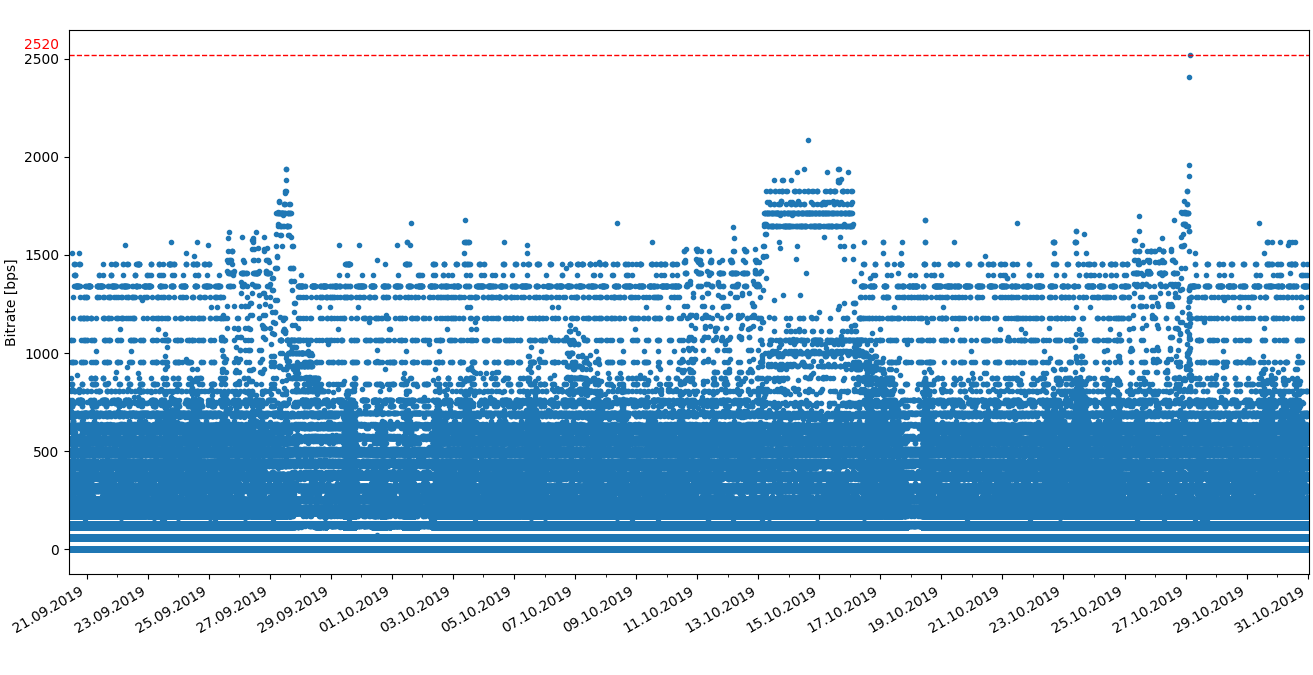
\includegraphics[width=1\textwidth]{03-dr-measured}
    \caption{Measured data rate in [bps] in RS485 network during long-term operation test}
    \label{fig:PacketLengthMeasuredAll}
\end{figure*}

Based on the frequency analysis given in Tab.~\ref{tab:FreqAnalysis} and IMA know-how, 19 Bytes length packets transmit sensor data, and 7 Bytes length packets are general aknowledgemets of IMA protocol. At least two packets are required to handle sensor data via RS485 network, i.e., one carrying sensor data and the other with ackowledgement.

%Fig. \ref{fig:PacketLengthMeasuredAll} shows 
%Two imporatnt characteristics are displayed, maximal length of packet (red colored dash line) and median length of packet (red colored solid line). It is determined by frequency analysis method as shown in Tab. \ref{tab:FreqAnalysis}. Average RS485 network channel traffic load is 6.38 pps, i.e., 0.85 Bps.
%shows lengths of captured packet  during
%Median of packet length is determined by using frequency analysis method, as shown in Tab. \ref{tab:FreqAnalysis}.
% 7,51 Byte --> simple arithmetic mean

During long term operation test, lengths of transmitted packets ($ l $) are captured with the accuracy of timestamps of a thousandth of a second. Then resampled to one second resolution interval using the sum function to easily represent achieved data as a bit rate in bit per second (bps),
Fig.~\ref{fig:PacketLengthMeasuredAll}.
Red colored dashed line (with value of 2520~bps) shows one second time interval in which a sum of captured packets is transported in RS485 network. It shows, based on detailed knowledge of the IMA protocol, less than 20\% of the RS485 network capacity is used. 
%This limit state is caused by data communication of two sensor nodes that occupied 2\% of capacity of used RS485 network.

To avoid RS485 network congestion the maximum number of sensor nodes $ S_{MAX} $ can be calculated as:
\begin{equation}
S_{MAX} = \frac{\frac{\frac{v_{485}}{B}}{l_{MAX}} - R}{P}
\label{equ:max-count-of-sensors}
\end{equation}

where:

\begin{tabular}{l @{  } l}
$v_{485}$ & 485 network data rate [bps]\\
 B        & bits to Byte \\
$l_{MAX}$ & maximal packet length \\
 R        & reserve of the data rate [\%]\\
 P        & number of packets to transmit sensor data \\
\end{tabular}

Considering above mentioned limits, desired reserves and RS485 data rates, the maximum number of sensor nodes simultaneously transmitting their data on RS485 network is calculated, Tab. \ref{tab:max-sensor-nodes}.

Values for calculation are:

\begin{tabular}{l @{ $=$ } l}
$v_{485}$ & RS485 network data rate \\
 B        & 8 \\
$l_{MAX}$ & 40 \\
 P        & 2 \\
\end{tabular}

% todo: this table makes error
% \begin{table}[ht]
% \centering
% \footnotesize
% \caption{Maximum number of sensor nodes simultaneously transmitting their data in RS485 network with desired reserve}
% \begin{tabular}{r|rrrr}
% \multicolumn{1}{c|}{\textbf{RS485}}     & \multicolumn{4}{c}{\multirow{2}{*}{\textbf{Reserve} $R$}}\\
% \multicolumn{1}{c|}{\textbf{data rate}} &   \\
% $v_{485}$ {[bps]}  &	0 \%	&	10 \%	&	20 \%	&	30 \%  \\ \hline
%   1200~~~ &    1	&    1	&    1	&    1 \\
%   2400~~~ &    3	&    3	&    3	&    2 \\
%   4800~~~ &    7	&    6	&    6	&    5 \\
%   9600~~~ &   15	&   13	&   12	&   10 \\
%  19200~~~ &   30	&   27	&   24	&   21 \\
%  38400~~~ &   60	&   54	&   48	&   42 \\
%  57600~~~ &   90	&   81	&   72	&   63 \\
% 115200~~~ &  180	&  162	&  144	&  126 \\
% 230400~~~ &  360	&  324	&  288	&  252 \\
% 460800~~~ &  720	&  648	&  576	&  504 \\
% 921600~~~ & 1440	& 1296	& 1152	& 1008 \\
% \end{tabular}
% \label{tab:max-sensor-nodes}
% \end{table}

For example, WSN can connect up to 162 sensor nodes that work in RS485 network with a 115200~bps data rate and 10 \% reserve, or up to 126 sensor nodes with a 115200~bps data rate and 30 \% reserve. The results also show, one floor block of university building, i.e., one RS485 network, can operates dozens of sensors with sufficient reserve protecting the access control system from malfunction.   


%%%%%%%%%%%%%%%%%%%%%%%%%%%%%%%%%%%%%%%%%%%%%%%%%%%%%%%%%%%%%%%%%%%%%%%%%%%%%%%%%%%%%%%
%       NOT USED
%%%%%%%%%%%%%%%%%%%%%%%%%%%%%%%%%%%%%%%%%%%%%%%%%%%%%%%%%%%%%%%%%%%%%%%%%%%%%%%%%%%%%%%
% The heavy traffic test simulates data transmission in the RS485 network as evidence of theoretically calculated values as shown in Tab \ref{tab:max-sensor-nodes}.

% \begin{figure}[!ht]
    % \centering
    % 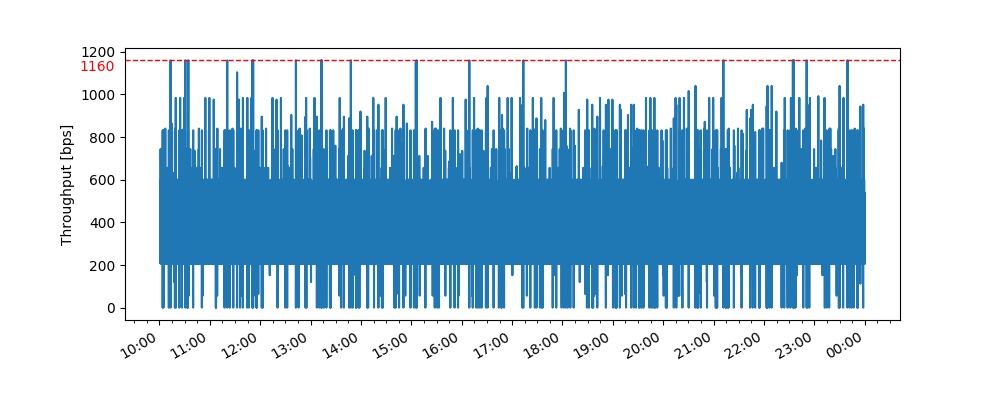
\includegraphics[width=.5\textwidth]{03-tp-simul}
    % \caption{RS485 datarates in simulation of heavy data traffic}
    % \label{fig:heavySimulation}
% \end{figure}

% This test simulated the transmission of more than 190~000 commands from 300 sensor nodes every 5 minutes simultaneously for 12 hours time period. The highest datarate achieved during simulation is 1160~bps, Fig \ref{fig:heavySimulation} red dashed line.

%!!! Tady to mozna chce frekvencni analyzu GW, at vis, jak jsou dlouhe pakety, pak nemusis hadat, nebo napis, ze max. delka je 19 bytů.

%Considering the worst case, ie packets with length of 40 Bytes, we have analytically calculated the maximum number of sensors a network can transmit based on the network transmission rate.

%\textbf{!!! Limit RS485: up to 32 transceivers on the serial bus !!! My vsak mame senzory pres LoRa ...Jo, ale to je fyzicky, to splnujeme, mame jich 13 :-)}
%datasheet: https://www.sparkfun.com/datasheets/Components/General/sp3485CN-LTR.pdf

%Space for peaks 10\% --> maximum packet rate is 324 pps
%Data measured in testing procedure shows Fig.

%\begin{table}[h]
%\centering
%\footnotesize
%\caption{Simple analytics of measured data}
%\begin{tabular}{lr}
%\textbf{Packet length} & \textbf{Bytes} \\ \hline
%Minimum   &   7 B     \\
%Maximum   &  40 B     \\
%mean      &   7,51 B  \\
%Median    &   7 B     \\
%\end{tabular}
%\label{tab: simple-analytics}
%\end{table}


%---
% tabulka, rezervy 10%, 30% ...
% Zjistit kolik sensoru muze byt na sbernici 485.
% popis os co  je co

% \chapter{Conclusions}
\chapter{Závěr}

In this paper, the conditions of extending an existing access control system running in an industry standardized RS485 network with a wireless sensor network based on LoRaWAN single-channel mode is discussed. 
Design of wireless sensor network is performed, i.e., the sensor nodes and one single-channel gateway based on LoRaWAN protocol are designed. The gateway represents a type of CKP device connected to the RS485 network, therefore is supports the existing protocol in the RS485 network. A long-term operation measurement is performed in one university floor infrastructure consisting of twelve CKP devices (pairs of card reader and door lock) and one gateway. Frequency analysis of packet lengths is performed and the biggest value of packet length is considered as well as the reserve of the RS485 data rate in order to protect the access control system from malfunction. 
Maximum number of wireless sensor nodes simultaneously transmitting data RS485 network is calculated in dependence on RS485 data rate and the reserve of data rate, e.g., 81 sensor nodes that work in RS485 network with a 57600~bps data rate and 10 \% reserve. This number of sensor nodes significantly exceeds the actual needs of the sensor nodes on one floor block of university building. Therefore we can state that WSN is suitable for smart metering applications.



%%%%%%%%%%%%%%%%%%%%%%%%%%%%%%%%%%%%%%%%%%%%%%%%
\bibliographystyle{amsalpha}
\bibliographystyle{csn690}
\bibliography{mybibliographyfile}
\begin{thebibliography}{9}
%%%%%%%%%%%%%%%%%%%%%%%%%%%%%%%%%%%%%%%%%%%%%%%%%%%%%%%%%%%%%%%



\bibitem[1]{nucleoST}
\textit{
NUCLEO-L073RZ.
}
ST Microelectronics
[Online]. Available:
\url{
https://www.st.com/en/evaluation-tools/nucleo-l073rz.html
}
[Accessed: 20-Sep-2019].

%___________________

\bibitem[2]{nucleoMbed}
\textit{
NUCLEO-L073RZ
}
ARM Mbed.
[Online]. Available:
\url{
https://os.mbed.com/platforms/ST-Nucleo-L073RZ/
}
[Accessed: 20-Sep-2019].

%___________________

\bibitem[3]{RFM95w}
\textit{
RFM95/96/97/98(W) - Low Power Long Range Transceiver Module}.
HopeRF electronic.
V1.0.
[Online]. Available:
\url{
http://wiki.dragino.com/index.php?title=Lora_Shield
}
[Accessed: 20-Sep-2019].

%___________________


\bibitem[4]{draginoWiki}
\textit{
Lora Shield.
}
Dragino.
[Online]. Available:
\url{
http://wiki.dragino.com/index.php?title=Lora_Shield
}
[Accessed: 20-Sep-2019].

%___________________


\bibitem[5]{AESlib}
\textit{
tiny-AES128-C
}
bitdust.
[Online]. Available:
\url{
https://github.com/bitdust/tiny-AES128-C
}
[Accessed: 20-Sep-2019].

%___________________


\bibitem[6]{CMAClib}
\textit{
openpana.
}
OpenPANA.
[Online]. Available:
\url{
https://github.com/OpenPANA/openpana
}
[Accessed: 20-Sep-2019].

%___________________


\bibitem[7]{rs485tr}
\textit{
SparkFun Transceiver Breakout - RS-485
}
Sparkfun.
[Online]. Available:
\url{
https://www.sparkfun.com/products/10124
}
[Accessed: 20-Sep-2019].


%___________________


\bibitem[8]{lwSpec}
\textit{
LoRaWAN Specification
}.
LoRa Alliance.
v1.1.
Sparkfun.
[Online]. Available:
\url{
https://lora-alliance.org/resource-hub/lorawantm-specification-v11
}
[Accessed: 20-Sep-2019].


%___________________


\bibitem[9]{lwSecur}
Robert Miller.
\textit{
LoRa Security
Building a Secure LoRa Solution.
}
MWR Labs Whitepaper.
[Online]. Available:
\url{
https://labs.mwrinfosecurity.com/assets/BlogFiles/mwri-LoRa-security-guide-1.2-2016-03-22.pdf
}
[Accessed: 20-Sep-2019].




% -------------------------
\bibitem[10]{accessControlSystem_eiprocus}
% \textit{

% }

[Online]. Available:
\url{
https://www.elprocus.com/understanding-about-types-of-access-control-systems/
}
[Accessed: 9-Sep-2019].


% -------------------------
\bibitem[11]{high density LPWAN}
% \textit{

% }

[Online]. Available:
\url{
https://ieeexplore.ieee.org/stamp/stamp.jsp?tp=&arnumber=8678997
}
[Accessed: 9-Sep-2019].

% -------------------------
\bibitem[12]{IoT cisco study}
% \textit{

% }

[Online]. Available:
\url{
https://blogs.cisco.com/innovation/the-internet-of-things-5-predictions-for-2018
}
[Accessed: 9-Sep-2019].

% % -------------------------
\bibitem[2]{IoT cisco study 02}
% \textit{

% }

[Online]. Available:
\url{
https://www.cisco.com/c/dam/en_us/about/ac79/docs/innov/IoT_IBSG_0411FINAL.pdf
}
[Accessed: 9-Sep-2019].

% % -------------------------
% \bibitem[2]{2}
% \textit{

% }

% [Online]. Available:
% \url{

% }
% [Accessed: 9-Sep-2019].

% % -------------------------
% \bibitem[2]{2}
% \textit{

% }

% [Online]. Available:
% \url{

% }
% [Accessed: 9-Sep-2019].

% % -------------------------
% \bibitem[2]{2}
% \textit{

% }

% [Online]. Available:
% \url{

% }
% [Accessed: 9-Sep-2019].

% % -------------------------
% \bibitem[2]{2}
% \textit{

% }

% [Online]. Available:
% \url{

% }
% [Accessed: 9-Sep-2019].





\end{thebibliography}

%\appendix


\end{document}ß